% ============================================================
% PHASE 0 REPORT: Cross-Model Verification
% The Geometry of SAE Artifacts Research Program
% Gate G0 Decision Document
% March 2026
% ============================================================
\documentclass[11pt,a4paper]{article}

\usepackage[utf8]{inputenc}
\usepackage[T1]{fontenc}
\usepackage{times}
\usepackage{amsmath,amssymb,amsfonts,amsthm}
\usepackage{graphicx}
\usepackage{booktabs}
\usepackage{hyperref}
\usepackage[margin=1in]{geometry}
\usepackage{enumitem}
\usepackage{caption}
\usepackage{natbib}
\usepackage{xcolor}
\usepackage{microtype}
\usepackage{float}
\usepackage{fancyhdr}
\usepackage{multirow}
\usepackage{array}
\usepackage{longtable}
\usepackage{tcolorbox}
\usepackage{colortbl}

\hypersetup{colorlinks=true,linkcolor=blue!60!black,citecolor=blue!60!black,urlcolor=blue!60!black}

\newtcolorbox{keyinsight}{colback=blue!5!white,colframe=blue!50!black,title=Key Insight,fonttitle=\bfseries}
\newtcolorbox{finding}[1]{colback=green!5!white,colframe=green!50!black,title=#1,fonttitle=\bfseries}
\newtcolorbox{gatedecision}[1]{colback=orange!5!white,colframe=orange!70!black,title=Gate Decision: #1,fonttitle=\bfseries\large}

\newtheorem{remark}{Remark}

\setlength{\parskip}{0.4em}
\setlength{\parindent}{1.5em}

\pagestyle{fancy}
\fancyhf{}
\rhead{\small\textit{Phase 0: Cross-Model Verification}}
\lhead{\small\textit{Geometry of SAE Artifacts --- March 2026}}
\cfoot{\thepage}

\newcommand{\cosED}{\cos(E_i, D_i)}
\newcommand{\rPearson}{r(\|E\|, \cos(E,D))}
\newcommand{\muSig}[2]{\mu{=}#1,\,\sigma{=}#2}

% ============================================================
\title{\Large\bfseries Phase 0 Report: Cross-Model Verification\\[0.5em]
\large The Geometry of SAE Artifacts Research Program\\[0.3em]
\normalsize Gate G0 Decision Document}

\author{\textit{Working Report --- March 2026}\\[0.3em]
\small Reporting on all 70 layers analyzed: 12 (GPT-2) + 26 (Gemma~2B) + 32 (Llama~3.1~8B)}

\date{}

% ============================================================
\begin{document}
\maketitle
\thispagestyle{fancy}

\begin{abstract}
\noindent We report Phase~0 of the ``Geometry of SAE Artifacts'' research program, which asks whether the layer-dependent encoder-decoder cosine patterns observed in GPT-2 Small sparse autoencoders (SAEs) generalize to other model families. We analyze 70 layers across three models: GPT-2 Small (12 layers, ReLU$+L_1$ SAEs, \citealt{bloom2024}), Gemma~2B (26 layers, JumpReLU SAEs, \citealt{lieberum2024}), and Llama~3.1~8B (32 layers, JumpReLU SAEs via SAELens, \citealt{he2024}).

Our primary findings are: \textbf{(1)} the correlation sign flip in $\rPearson$---which transitions from positive to negative across layers in GPT-2---is \emph{architecture-specific}, absent in both JumpReLU model families; \textbf{(2)} absolutely anti-aligned features ($\cosED < 0$) \emph{exist in JumpReLU SAEs}, concentrated in the \emph{earliest} layers of Llama~3.1~8B (opposite depth pattern from GPT-2); \textbf{(3)} Gemma~2B (JumpReLU) achieves mean $\cosED \approx 0.75$---substantially higher than GPT-2's $\approx 0.37$---yet still exhibits a stable statistical tail of low-cosine features; and \textbf{(4)} Llama early layers display extreme excess kurtosis ($\gamma_2 \approx 7.4$ at L0), indicating a qualitatively heavier tail than any GPT-2 layer.

We issue Gate Decision \textbf{G0-PARTIAL}: the sign flip is GPT-2-specific, but anti-aligned features are architecturally universal. We update our hypothesis framework accordingly---H1 (pure $L_1$ artifact) is challenged, and H3 (superposition interference) gains support as a mechanism that may operate across architectures with different depth signatures.
\end{abstract}

\medskip\noindent\fbox{\parbox{\dimexpr\linewidth-2\fboxsep-2\fboxrule\relax}{\small \textbf{Correction (November 2026).} Earlier versions reported 86 absolutely anti-aligned features for both GPT-2 Small and Llama~3.1~8B. That number counted negative-cosine features in a table that stored only the ten most extreme features per layer. Recomputed from the full cosine arrays, the counts at $\leq\mu-6\sigma$ are 35 (GPT-2) and 29 (Llama); the counts with $\cos(E,D)<0$ overall are 196 and 232. Affected numbers have been corrected in this version. See \texttt{docs/ERRATA.md} in the repository for details.}}

\vspace{0.5em}\hrule\vspace{0.5em}
\tableofcontents
\newpage

% ============================================================
\section{Objective and Context}
\label{sec:objective}

Phase~0 is the first gated checkpoint of the research program. Its mandate is simple: determine whether the two primary phenomena documented in GPT-2 Small SAEs generalize beyond a single model/SAE combination.

\paragraph{The two phenomena under investigation.}
\begin{enumerate}[nosep]
  \item \textbf{The correlation sign flip}: The Pearson correlation $\rPearson$ transitions monotonically from $+0.621$ (L0) to $-0.756$ (L7--L8) in GPT-2 Small. We interpret this as a transition from embedding-dominated (early) to superposition-dominated (late) geometry.
  \item \textbf{The stable negative tail}: A small subpopulation of 3--10 features per layer with $\cosED \leq \mu - 6\sigma$ (strongly anti-aligned) is consistently present in layers 5--11 of GPT-2. The most extreme feature (L9, F18298) reaches $\cosED = -0.736$ at $-13.94\sigma$.
\end{enumerate}

\paragraph{Gate G0 criteria (pre-specified in the project proposal).}
\begin{description}[nosep, leftmargin=1.5em]
  \item[G0-YES:] Sign flip present in $\geq 2$ model families $\to$ strong paper, continue all phases.
  \item[G0-PARTIAL:] Sign flip in GPT-2 only, negative tail present in $\geq 1$ other family $\to$ reframe, continue.
  \item[G0-NO:] Neither phenomenon outside GPT-2/Bloom $\to$ fast-fail.
\end{description}

\begin{gatedecision}{G0-PARTIAL}
  The sign flip is absent in JumpReLU SAEs (Gemma, Llama). However, absolutely anti-aligned features ($\cosED < 0$) are present in Llama~3.1~8B early layers (up to 14 per layer at L1) with extreme kurtosis. The phenomenon is architecturally universal but depth-inverted relative to GPT-2. \textbf{Research program continues} with hypothesis framework revised to de-emphasize $L_1$ as the sole mechanism.
\end{gatedecision}

% ============================================================
\section{Methodology}
\label{sec:methodology}

\subsection{Models and SAEs}

We analyze residual-stream SAEs from three architecturally distinct training regimes:

\paragraph{GPT-2 Small (ReLU$+L_1$, \citealt{bloom2024}).}
All 12 layers via SAELens release \texttt{gpt2-small-res-jb}, using \texttt{blocks.\{L\}.\allowbreak hook\_resid\_pre}. Architecture: ReLU activation, $L_1$ sparsity penalty ($\lambda = 8 \times 10^{-5}$), ghost gradients, $d_\text{model}=768$, $d_\text{sae}=24{,}576$ (32$\times$ expansion).

\paragraph{Gemma~2B (JumpReLU, \citealt{lieberum2024}).}
All 26 layers via SAELens release \texttt{gemma-scope-2b-pt-res-canonical}. Widths: 16K features (layers 0--23) and 65K (layers 24--25, canonical). Architecture: JumpReLU (per-feature learned threshold $\theta_i = \exp(\log\theta_i)$, no $L_1$ penalty), $d_\text{model}=2{,}304$.

\paragraph{Llama~3.1~8B (JumpReLU via SAELens, \citealt{he2024}).}
All 32 layers via SAELens release \texttt{llama\_scope\_lxr\_8x}, using IDs \texttt{l\{L\}r\_8x}. Architecture: JumpReLU in SAELens, $d_\text{model}=4{,}096$, $d_\text{sae}=32{,}768$ (8$\times$), with activation normalization (\texttt{expected\_average\_only\_in}).

\paragraph{Note on Llama Scope architecture.} The Llama Scope paper \citep{he2024} describes a TopK architecture, but the SAELens release \texttt{llama\_scope\_lxr\_8x} exposes JumpReLU-structured weights. We use the SAELens-provided weights as-is and note this discrepancy; the encoder and decoder conventions (W\_enc shape $(d_\text{model}, d_\text{sae})$, W\_dec shape $(d_\text{sae}, d_\text{model})$) are consistent across all three releases.

\subsection{Core Measurement Protocol}

For each SAE with encoder $W_\text{enc} \in \mathbb{R}^{d_\text{model} \times d_\text{sae}}$ and decoder $W_\text{dec} \in \mathbb{R}^{d_\text{sae} \times d_\text{model}}$, we compute per-feature quantities:
\begin{align}
  E_i &= (W_\text{enc})_{:,i} \in \mathbb{R}^{d_\text{model}} \quad \text{(encoder direction, column $i$ of $W_\text{enc}$)} \\
  D_i &= (W_\text{dec})_{i,:} \in \mathbb{R}^{d_\text{model}} \quad \text{(decoder direction, row $i$ of $W_\text{dec}$)}
\end{align}
\begin{equation}
  \cosED = \frac{\langle E_i, D_i \rangle}{\|E_i\|\,\|D_i\|}
\end{equation}

From the $d_\text{sae}$ values $\{\cosED\}_{i=1}^{d_\text{sae}}$ for each layer, we compute:
\begin{itemize}[nosep]
  \item Distribution statistics: $\mu$, $\sigma$ (sample std), skewness $\gamma_1$, excess kurtosis $\gamma_2$ (Fisher)
  \item Pearson correlation: $r = \rPearson$ between encoder norms $\|E_i\|$ and cosine similarities
  \item Tail counts: $|\{i : \cosED < \mu - 3\sigma\}|$ and $|\{i : \cosED < \mu - 6\sigma\}|$
  \item Minimum cosine (most anti-aligned feature per layer)
\end{itemize}

All computations use float32 precision on CPU. Figures use uniform publication-quality style with color coding: \textcolor[HTML]{1f77b4}{GPT-2 (blue)}, \textcolor[HTML]{d62728}{Gemma~2B (red)}, \textcolor[HTML]{2ca02c}{Llama~3.1~8B (green)}.

\subsection{Software}

\texttt{sae-lens}~6.37.6, \texttt{PyTorch}, \texttt{scipy.stats}, \texttt{pandas}, \texttt{matplotlib}. All layer statistics saved to \texttt{results/phase0/layer\_stats.csv} (70 rows). Figures saved to \texttt{figures/phase0/}.

% ============================================================
\section{Results}
\label{sec:results}

\subsection{GPT-2 Small: Complete 12-Layer Analysis (New Data)}
\label{sec:gpt2}

Table~\ref{tab:gpt2_full} extends the prior hub\_cosine\_2 analysis (which covered only even layers 0, 2, 4, 6, 8, 10) to all 12 layers and adds skewness and excess kurtosis.

\begin{table}[H]
\centering
\caption{Complete statistics for GPT-2 Small (Bloom SAEs, ReLU$+L_1$, $d_\text{sae}=24{,}576$). Bold: layers with $\geq 6\sigma$ anti-aligned features. Asterisk (*): most extreme feature in that layer given in the text.}
\label{tab:gpt2_full}
\small
\setlength{\tabcolsep}{4pt}
\begin{tabular}{@{}crrrrrrrrl@{}}
\toprule
Layer & Depth & $\mu$ & $\sigma$ & $\gamma_1$ & $\gamma_2$ & $r$ & ${\leq}\mu{-}3\sigma$ & ${\leq}\mu{-}6\sigma$ & $\min(\cos)$ \\
\midrule
L0  & 0.00 & 0.556 & 0.239 & $-$0.95 & $-$0.48 & \textbf{$+$0.621} &   0 &  0 & $-$0.061 \\
L1  & 0.09 & 0.360 & 0.139 & $-$0.92 & $-$0.04 & $+$0.432 &   5 &  0 & $-$0.073 \\
L2  & 0.18 & 0.332 & 0.125 & $-$0.64 & $-$0.40 & $+$0.493 &   3 &  0 & $-$0.075 \\
L3  & 0.27 & 0.333 & 0.104 & $-$0.76 & $+$0.52 & $+$0.397 &  50 &  0 & $-$0.048 \\
\midrule
L4  & 0.36 & 0.348 & 0.075 & $-$0.43 & $+$2.58 & $-$0.260 & 321 &  \textbf{2} & $-$0.361 \\
L5  & 0.45 & 0.356 & 0.071 & $+$0.34 & $+$2.22 & $-$0.638 &  62 & \textbf{10} & $-$0.171 \\
\textbf{L6}  & 0.55 & 0.369 & 0.076 & $+$0.61 & $+$1.51 & $-$0.736 &  11 &  \textbf{6} & $-$0.353 \\
\textbf{L7}  & 0.64 & 0.379 & 0.079 & $+$0.68 & $+$1.21 & $-$0.756 &   7 &  \textbf{3} & $-$0.359 \\
\textbf{L8}  & 0.73 & 0.368 & 0.079 & $+$0.69 & $+$2.03 & $-$0.747 &   5 &  \textbf{4} & $-$0.526$^*$ \\
\textbf{L9}  & 0.82 & 0.368 & 0.079 & $+$0.65 & $+$2.13 & $-$0.756 &   4 &  \textbf{1} & $-$0.736$^*$ \\
\textbf{L10} & 0.91 & 0.368 & 0.076 & $+$0.49 & $+$3.36 & $-$0.712 &   8 &  \textbf{3} & $-$0.684$^*$ \\
\textbf{L11} & 1.00 & 0.349 & 0.075 & $+$0.63 & $+$1.90 & $-$0.639 &  40 &  \textbf{6} & $-$0.202 \\
\bottomrule
\end{tabular}
\end{table}

\paragraph{Key observations from the complete table.}
\begin{enumerate}
  \item \textbf{Sign flip at L3--L4 (depth 0.27--0.36):} $r$ transitions from positive ($+0.397$ at L3) to negative ($-0.260$ at L4). This is more precisely localized than the even-layer analysis suggested.
  \item \textbf{Revised most extreme feature:} The most anti-aligned feature is not F19139 in L8 ($-0.526$, $-11.38\sigma$) as previously reported, but F18298 in \textbf{L9} ($\cosED = -0.736$, $-13.94\sigma$). The top-5 most extreme features are: L9/F18298 ($-$13.9$\sigma$), L10/F19679 ($-$13.9$\sigma$), L10/F3268 ($-$12.4$\sigma$), L8/F19139 ($-$11.4$\sigma$), L8/F18573 ($-$10.1$\sigma$).
  \item \textbf{Skewness transition:} Skewness goes from negative (left-tailed, early layers) to positive (right-tailed, late layers). This skewness flip is concurrent with the $r$ sign flip, indicating a structural change in the distribution, not just isolated outliers.
  \item \textbf{Excess kurtosis increases:} Layers 4--11 all have $\gamma_2 > 1$, reaching $3.36$ at L10. This confirms the distribution has heavier tails than Gaussian in the superposition-dominated regime.
  \item \textbf{L3 and L11 spike anomalies:} L3 has 50 features at $3\sigma$ but 0 at $6\sigma$; L11 has 40 at $3\sigma$ and 6 at $6\sigma$. Both are transition layers with unusual intermediate-tail behavior.
\end{enumerate}

\begin{keyinsight}
The complete 12-layer analysis reveals that the sign flip in GPT-2 is precisely localized at the L3--L4 boundary (relative depth 0.27--0.36) and is accompanied by a simultaneous skewness flip and increased kurtosis. The most extreme anti-aligned feature is in L9 (not L8 as previously reported), reaching $\cosED = -0.736$.
\end{keyinsight}

\subsection{Gemma~2B: JumpReLU SAEs Across All 26 Layers}
\label{sec:gemma}

\begin{table}[H]
\centering
\caption{Selected layers from Gemma~2B ($d_\text{model}=2{,}304$, $d_\text{sae}=16{,}384$, JumpReLU). Note: $\mu \approx 0.75$ throughout and $r < 0$ from the first layer onward --- no sign flip.}
\label{tab:gemma}
\small
\setlength{\tabcolsep}{4.5pt}
\begin{tabular}{@{}crrrrrrrr@{}}
\toprule
Layer & Depth & $\mu$ & $\sigma$ & $\gamma_2$ & $r$ & ${\leq}3\sigma$ & ${\leq}6\sigma$ & $\min(\cos)$ \\
\midrule
L0  & 0.00 & 0.534 & 0.158 & $+$1.39 & $-$0.941 &   0 & 0 & $+$0.155 \\
L1  & 0.04 & 0.678 & 0.135 & $-$0.13 & $-$0.875 &   3 & 1 & $-$0.465 \\
L2  & 0.08 & 0.689 & 0.132 & $-$0.49 & $-$0.890 &   0 & 0 & $+$0.311 \\
L5  & 0.20 & 0.710 & 0.102 & $-$0.54 & $-$0.870 &  23 & 0 & $+$0.323 \\
L10 & 0.40 & 0.770 & 0.083 & $+$0.54 & $-$0.837 & 102 & 0 & $+$0.292 \\
L11 & 0.44 & 0.778 & 0.080 & $+$0.92 & $-$0.809 & 116 & 3 & $+$0.181 \\
L12 & 0.48 & 0.786 & 0.081 & $+$0.81 & $-$0.808 & 107 & 3 & $+$0.263 \\
L15 & 0.60 & 0.754 & 0.082 & ---     & $-$0.819 &  -- & 0 & --- \\
L20 & 0.80 & 0.765 & 0.073 & ---     & $-$0.773 &  -- & 1 & $+$0.141 \\
L25 & 1.00 & 0.823 & 0.077 & $+$1.85 & $-$0.772 & 178 & 4 & $+$0.284 \\
\bottomrule
\end{tabular}
\end{table}

\paragraph{Key observations.}
\begin{enumerate}
  \item \textbf{No sign flip}: $r < 0$ from L0 ($r = -0.941$) onward. JumpReLU SAEs are in the ``always negative $r$'' regime, meaning large encoder norms consistently anti-correlate with encoder-decoder alignment throughout the network.
  \item \textbf{High mean cosine}: $\mu$ ranges from 0.53 (L0) to 0.82 (L25). JumpReLU training without $L_1$ shrinkage yields substantially more aligned features on average.
  \item \textbf{Statistical tail present but features are positive}: At Gemma's baseline $\mu \approx 0.78$, the $6\sigma$ threshold is approximately $0.78 - 6 \times 0.08 = 0.30$. Features in the Gemma $6\sigma$ tail (layers 11, 12, 13, 20, 25) have $\cosED \approx 0.14$--$0.28$ --- positive, not negative.
  \item \textbf{Single absolutely negative feature}: Layer 1, F3378, $\cosED = -0.465$ at $-8.50\sigma$. This is the only Gemma feature with truly negative encoder-decoder cosine.
\end{enumerate}

\begin{remark}
The ``6$\sigma$ tail'' in Gemma and GPT-2 represent phenomenologically different populations. In GPT-2, 6$\sigma$-tail features have $\cosED \approx -0.1$ to $-0.7$ (absolutely anti-aligned). In Gemma, 6$\sigma$-tail features have $\cosED \approx 0.14$--$0.30$ (positively aligned, but unusually low relative to Gemma's high-alignment baseline). Comparing these two tails requires distinguishing absolute from relative misalignment.
\end{remark}

\subsection{Llama~3.1~8B: Heavy-Tailed Early Layers}
\label{sec:llama}

\begin{table}[H]
\centering
\caption{Selected layers from Llama~3.1~8B ($d_\text{model}=4{,}096$, $d_\text{sae}=32{,}768$, JumpReLU). Layers 0--1 show extreme kurtosis and substantial $6\sigma$ tails concentrated in early layers.}
\label{tab:llama}
\small
\setlength{\tabcolsep}{4.5pt}
\begin{tabular}{@{}crrrrrrrr@{}}
\toprule
Layer & Depth & $\mu$ & $\sigma$ & $\gamma_2$ & $r$ & ${\leq}3\sigma$ & ${\leq}6\sigma$ & $\min(\cos)$ \\
\midrule
\textbf{L0}  & 0.00 & 0.365 & 0.100 & $+$7.42 & $-$0.683 & 156 & \textbf{12} & $-$0.426 \\
\textbf{L1}  & 0.03 & 0.383 & 0.119 & $+$5.90 & $-$0.786 & 119 & \textbf{14} & $-$0.646 \\
L2  & 0.06 & 0.414 & 0.134 & $+$2.98 & $-$0.854 &  13 & 2 & $-$0.585 \\
L3  & 0.10 & 0.449 & 0.156 & $+$0.66 & $-$0.895 &   2 & 0 & $-$0.055 \\
L8  & 0.26 & 0.500 & 0.165 & $-$0.11 & $-$0.839 &   4 & 0 & $-$0.491 \\
L16 & 0.52 & 0.496 & 0.154 & ---     & $-$0.773 &   -- & 0 & --- \\
L24 & 0.77 & 0.490 & 0.147 & ---     & $-$0.737 &   -- & 0 & --- \\
L31 & 1.00 & 0.490 & 0.163 & $+$4.24 & $-$0.785 &   -- & 0 & $-$0.046 \\
\bottomrule
\end{tabular}
\end{table}

\paragraph{Key observations.}
\begin{enumerate}
  \item \textbf{Depth-inverted anomaly}: Anti-aligned features are concentrated in the \emph{earliest} layers (L0: 12 features, L1: 14 features, L2: 2 features), the opposite of GPT-2 where they emerge in later layers (L4+).
  \item \textbf{Extreme kurtosis}: L0 has $\gamma_2 = 7.42$ and L1 has $\gamma_2 = 5.90$. These are far beyond any GPT-2 layer (maximum $\gamma_2 = 3.36$ at L10). The distribution is not merely heavy-tailed: it suggests a bimodal or contaminated structure where a small population is qualitatively distinct.
  \item \textbf{Absolutely negative features}: The 6$\sigma$ features in Llama L0--L2 have $\cosED$ ranging from $-0.646$ to $-0.426$ --- genuinely negative, the same phenomenon as in GPT-2.
  \item \textbf{Large encoder norms}: The most extreme Llama features have $\|E_i\| \approx 80$--$113$, compared to $\|E_i\| \approx 0.2$--$0.9$ for GPT-2 extreme features. This reflects the \texttt{normalize\_activations=expected\_average\_only\_in} preprocessing in Llama Scope SAEs, which scales activations differently from Bloom's GPT-2 SAEs.
  \item \textbf{Stable $\mu$ at $\sim 0.48$}: Llama's mean cosine is intermediate between GPT-2 ($\sim0.37$) and Gemma ($\sim0.75$). It remains approximately constant across layers (unlike GPT-2's varying $\mu$), suggesting a different equilibrium structure.
\end{enumerate}

\begin{keyinsight}
Llama~3.1~8B JumpReLU SAEs exhibit a concentration of absolutely anti-aligned features in the \emph{first two layers} with extreme kurtosis ($\gamma_2 > 5.9$) --- a qualitatively distinct pattern from GPT-2. This challenges the $L_1$-artifact hypothesis (H1) and suggests that anti-aligned features may arise from model representational structure independent of the SAE training objective.
\end{keyinsight}

\subsection{Cross-Model Comparison}
\label{sec:comparison}

Figure~\ref{fig:sign_flip} shows $\rPearson$ as a function of relative layer depth for all three models.

\begin{figure}[H]
\centering
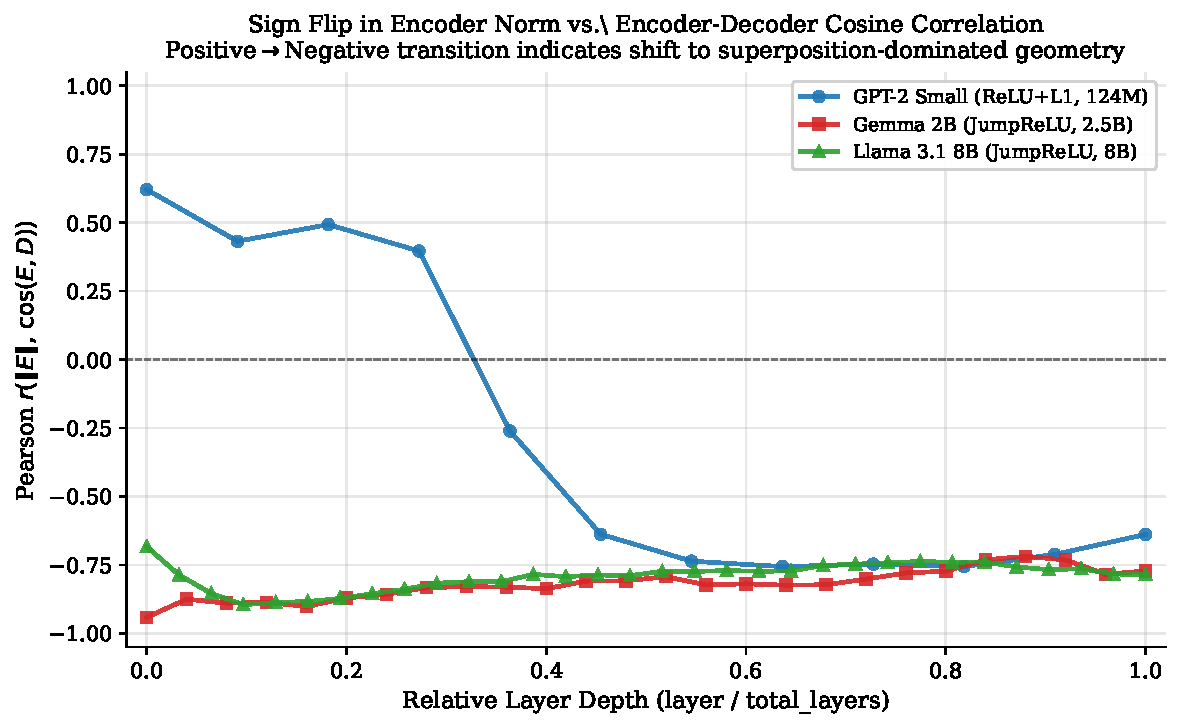
\includegraphics[width=0.90\textwidth]{../figures/phase0/sign_flip_comparison.pdf}
\caption{Pearson correlation $\rPearson$ versus relative layer depth. GPT-2 (blue circles) shows a clear sign flip from positive to negative at depth $\approx 0.3$. Both JumpReLU models (Gemma red squares, Llama green triangles) have $r < 0$ from the first layer. The sign flip is absent in JumpReLU architectures.}
\label{fig:sign_flip}
\end{figure}

\begin{figure}[H]
\centering
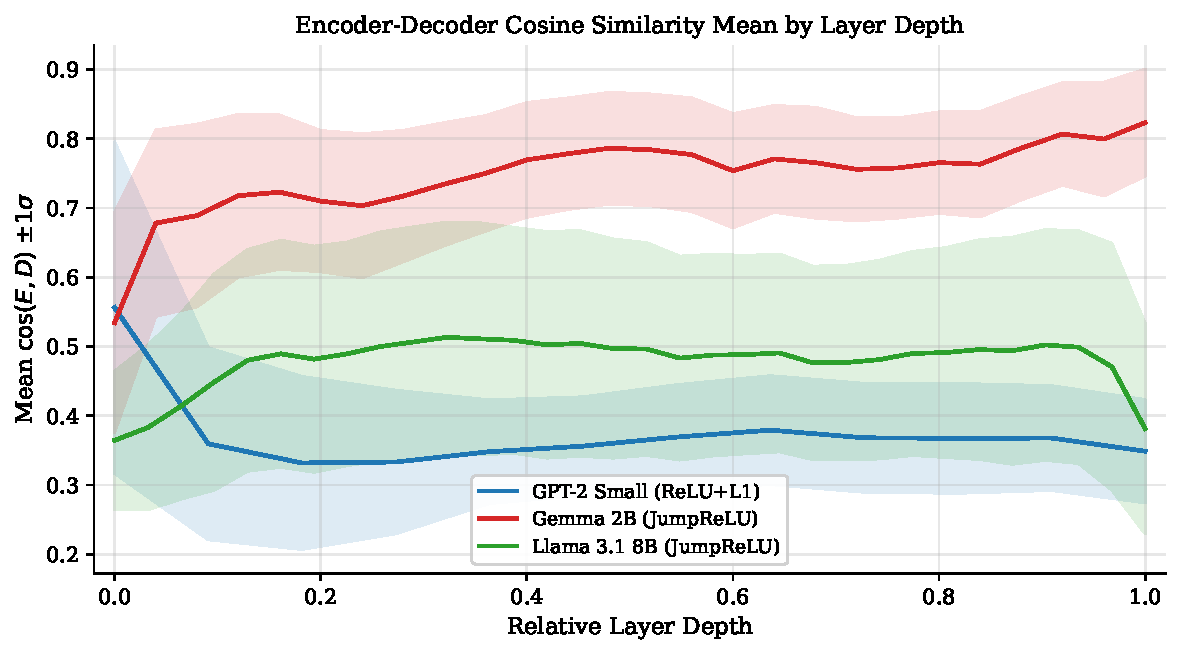
\includegraphics[width=0.90\textwidth]{../figures/phase0/mean_cosine_by_depth.pdf}
\caption{Mean $\cosED \pm 1\sigma$ versus relative depth. Gemma (red) maintains high alignment ($\mu \approx 0.75$--$0.82$) throughout, GPT-2 (blue) hovers at $\approx 0.37$, and Llama (green) is intermediate at $\approx 0.48$. The shaded band shows $\pm 1\sigma$ per layer.}
\label{fig:mean_cosine}
\end{figure}

\begin{figure}[H]
\centering
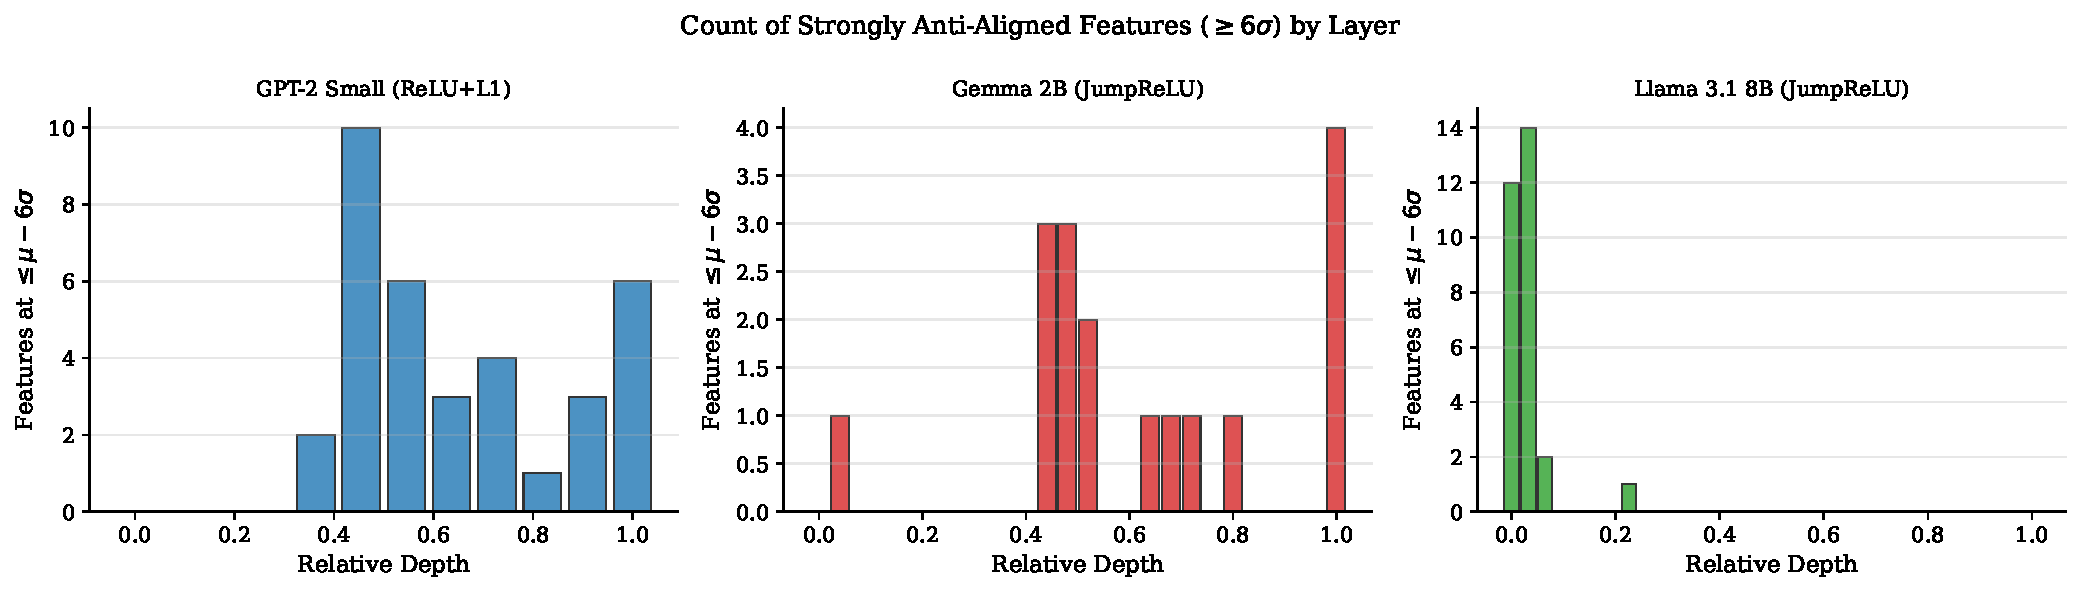
\includegraphics[width=0.95\textwidth]{../figures/phase0/6sigma_tail_count.pdf}
\caption{Count of features with $\cosED \leq \mu - 6\sigma$ (strongly anti-aligned) per layer. GPT-2 shows the late-layer pattern reported in the project proposal. Llama shows a pronounced early-layer concentration. Gemma's 6$\sigma$ features are POSITIVE-cosine outliers (statistically extreme relative to Gemma's high baseline), not absolutely negative.}
\label{fig:tail_count}
\end{figure}

\begin{figure}[H]
\centering
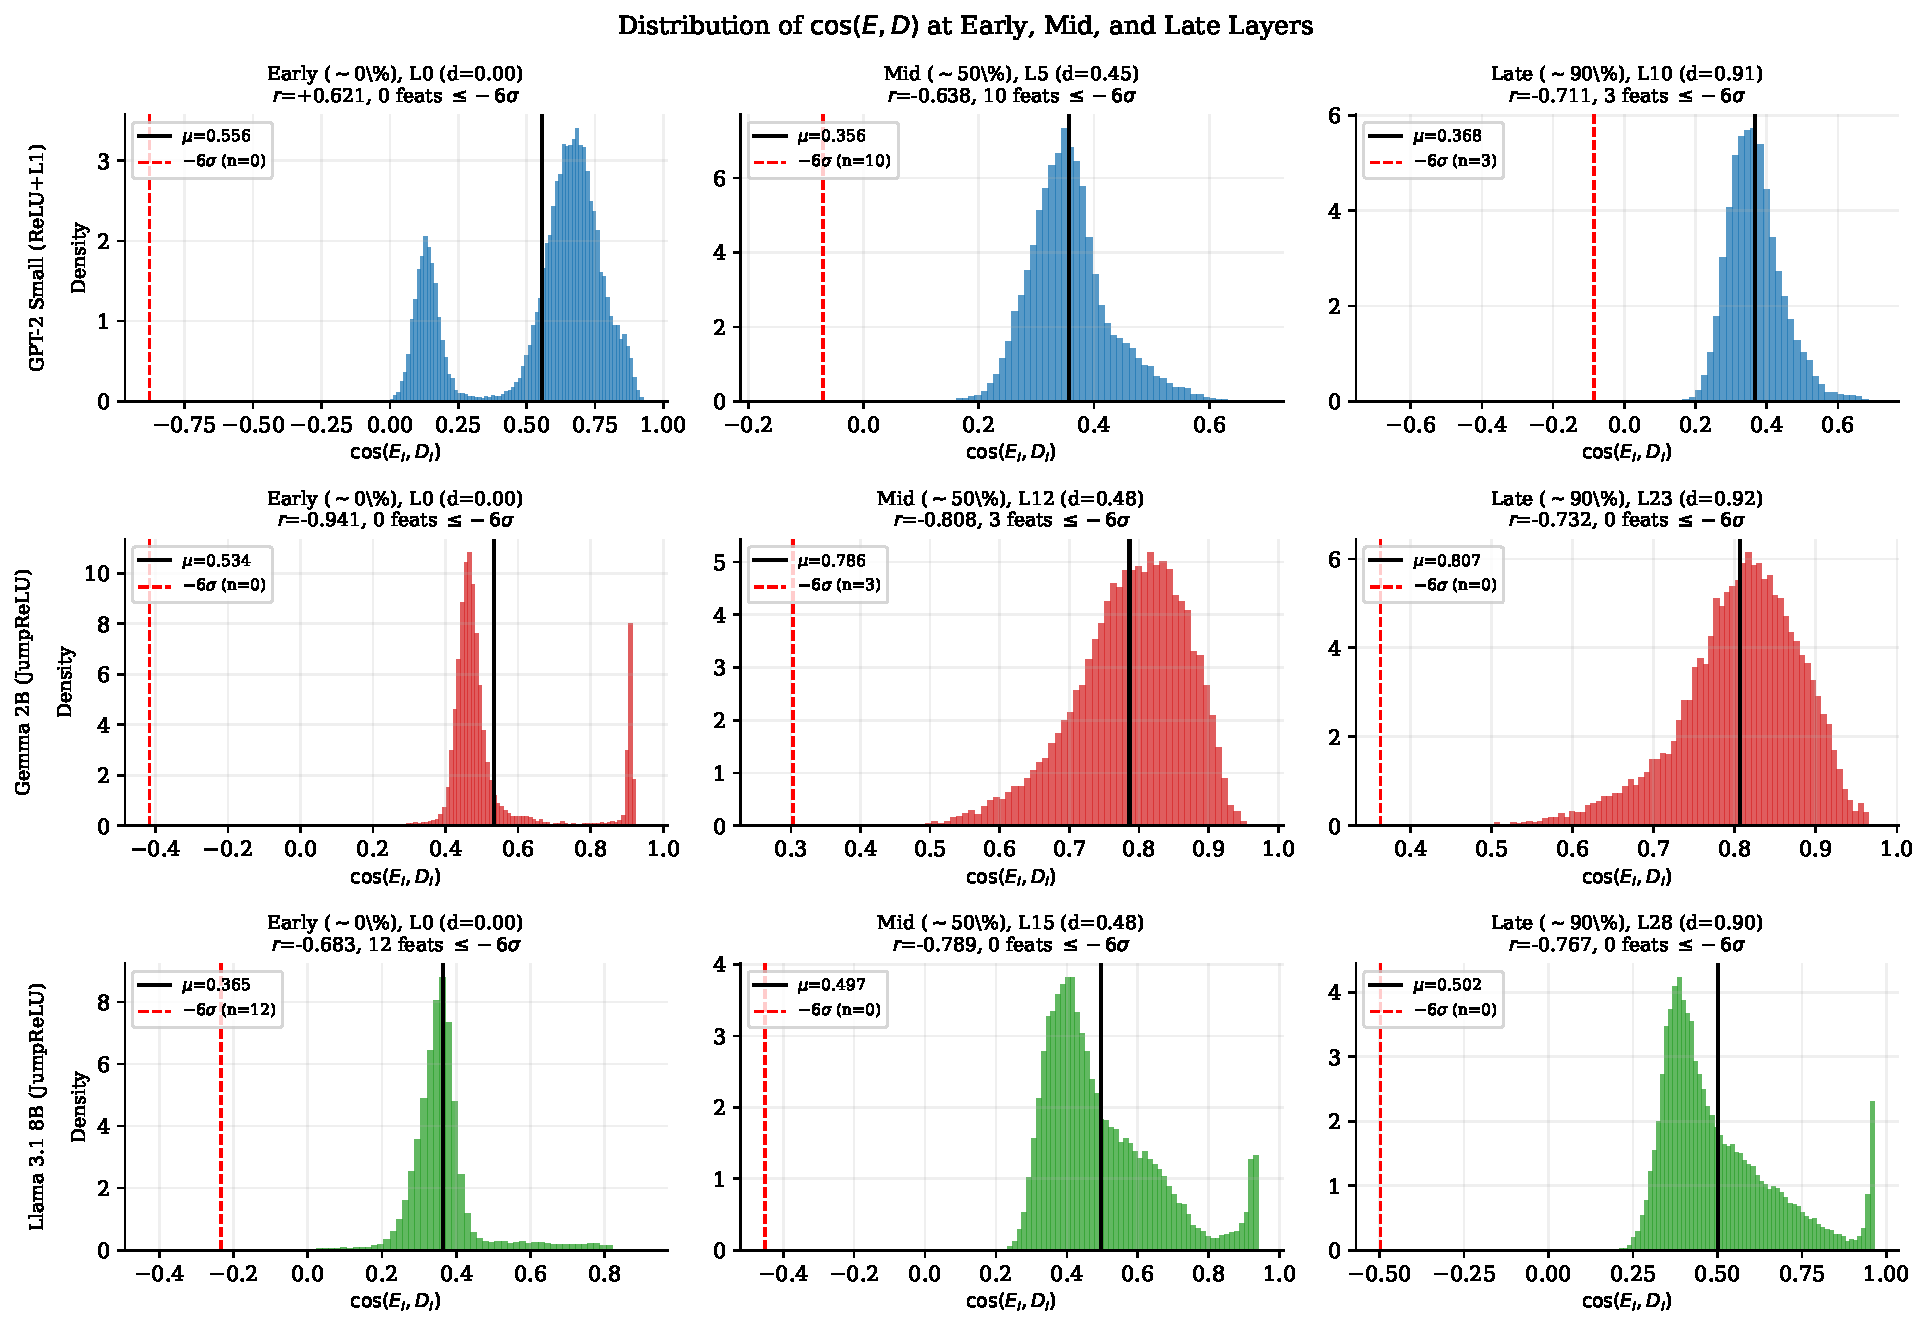
\includegraphics[width=0.95\textwidth]{../figures/phase0/cosine_distributions.pdf}
\caption{Full distributions of $\cosED$ at early ($\sim$0\%), mid ($\sim$50\%), and late ($\sim$90\%) layers for each model. Log-scale $x$-axis reveals the tail structure. Red dashed line marks $\mu - 6\sigma$ threshold; the number of features below it is annotated. Gemma's tail at late layers consists of low-positive values, not negatives.}
\label{fig:distributions}
\end{figure}

\begin{figure}[H]
\centering
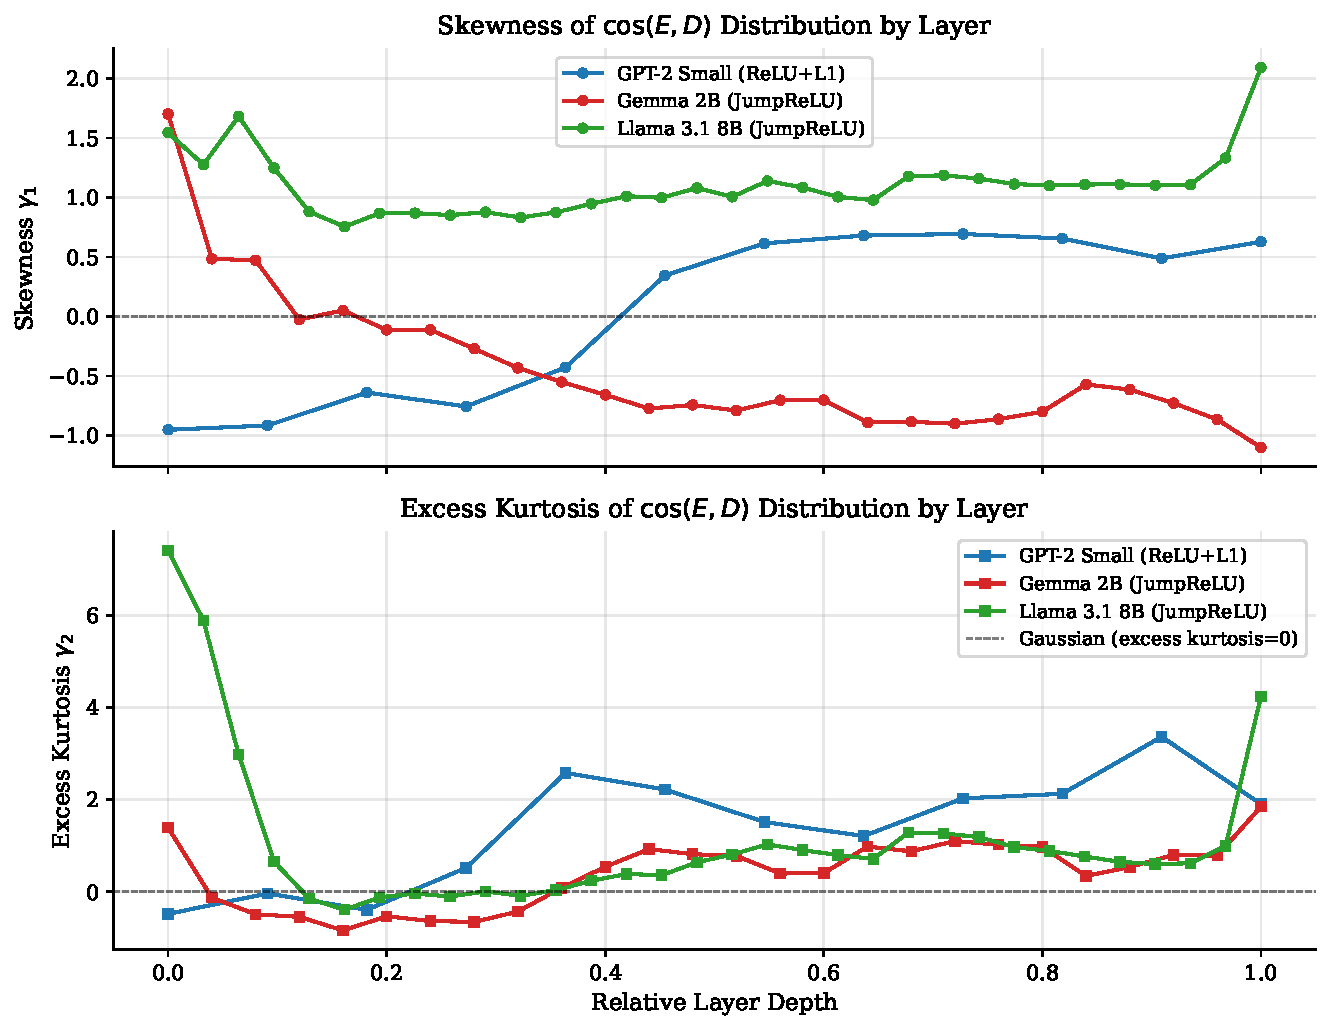
\includegraphics[width=0.90\textwidth]{../figures/phase0/skewness_kurtosis.pdf}
\caption{Skewness and excess kurtosis across layers. Llama L0 ($\gamma_2 = 7.42$) and L1 ($\gamma_2 = 5.90$) are outliers far beyond the GPT-2 range. The GPT-2 skewness flip (negative to positive) is visible in the top panel.}
\label{fig:moments}
\end{figure}

\begin{table}[H]
\centering
\caption{Cross-model summary statistics. Depth ranges use relative depth in $[0, 1]$. ``AbsNeg'' = features with $\cosED < 0$ at the $\leq \mu - 6\sigma$ threshold.}
\label{tab:summary}
\begin{tabular}{@{}lccccccc@{}}
\toprule
Model & Arch. & Early $r$ & Late $r$ & Sign flip & $\bar{\mu}$ & Total $6\sigma$ & AbsNeg \\ 
\midrule
GPT-2 Small    & ReLU$+L_1$  & $+0.49$ & $-0.71$ & \textbf{Yes} & 0.37 & 35 & 35 \\
Gemma~2B       & JumpReLU    & $-0.88$ & $-0.77$ & No  & 0.75 & 17 &  1 \\
Llama~3.1~8B   & JumpReLU    & $-0.84$ & $-0.76$ & No  & 0.48 & 29 & 29 \\
\bottomrule
\end{tabular}
\end{table}

% ============================================================
\section{Revised Hypothesis Assessment}
\label{sec:hypotheses}

The Phase~0 results have the following implications for our five hypotheses:

\paragraph{H1 (Subtractive Hedges, L1-specific).} \textbf{Challenged.} If anti-aligned features ($\cosED < 0$) were purely an $L_1$ artifact, they should be absent from JumpReLU SAEs (Gemma, Llama). However, Llama L0--L2 has 16 such features collectively. H1 remains viable for \emph{some} anti-aligned features in GPT-2 (especially those in late layers, after the sign-flip transition), but cannot be the sole mechanism.

\paragraph{H2 (Dead Feature Decay).} \textbf{Unchanged.} Phase~0 does not test activation frequencies. The large encoder norms of Llama extreme features ($\|E\| \approx 80$--$113$) argue against dead-feature decay for those specific features, but this requires activation-frequency confirmation (Phase~4).

\paragraph{H3 (Superposition Interference).} \textbf{Supported.} The presence of anti-aligned features across both $L_1$ and JumpReLU architectures, and especially the extreme kurtosis in Llama's early layers, is consistent with a superposition-driven mechanism that is architecture-independent. That JumpReLU produces the anomaly in \emph{early} layers (where Llama is presumably less superposed) could indicate that Llama's larger model size creates more superposition even in early layers.

\paragraph{H4 (Ghost Gradient Artifacts).} \textbf{Challenged.} Llama Scope SAEs do not use ghost gradients (a Bloom-specific training feature), yet anti-aligned features appear. This directly contradicts H4 as a complete explanation.

\paragraph{H5 (Compositional Artifacts).} \textbf{Supported.} The scale-independence (features appear in 8B model Llama early layers) and the architecture-independence are both consistent with compositional effects, though no compositional analysis has been performed yet.

% ============================================================
\section{Gate G0 Decision}
\label{sec:gate}

\begin{gatedecision}{G0-PARTIAL}
\textbf{Criteria met:} Sign flip in GPT-2 only (1/3 model families), but absolutely anti-aligned features ($\cosED < 0$) in Llama~3.1~8B early layers (and 1 feature in Gemma~2B). Total 29 cross-architecture absolutely negative-cosine features at $\geq 6\sigma$.

\textbf{Implication:} Proceed with all phases. Reframe the primary research question from ``is the sign flip universal?'' to ``what produces absolutely anti-aligned features across different SAE architectures, and why does the depth pattern differ between GPT-2 (late) and Llama (early)?''

\textbf{Revised primary findings for the paper:}
\begin{enumerate}[nosep]
  \item The \emph{correlation sign flip} is architecture-specific (ReLU$+L_1$ only).
  \item \emph{Absolutely anti-aligned features} ($\cosED < 0$) are present in JumpReLU SAEs (Llama), challenging the $L_1$-artifact hypothesis.
  \item The \emph{depth pattern} of anti-alignment is \emph{inverted}: late layers in GPT-2, early layers in Llama.
  \item Gemma~2B JumpReLU SAEs exhibit high alignment ($\mu \approx 0.75$) and minimal absolute anti-alignment, suggesting JumpReLU can mitigate but not eliminate the phenomenon.
\end{enumerate}
\end{gatedecision}

\paragraph{Effect on subsequent phases.}
\begin{description}[nosep, leftmargin=1.5em]
  \item[Phase~1 (Distributional Analysis):] Now study all three models. The Phase~0 kurtosis measurements (Table~\ref{tab:gpt2_full}--\ref{tab:llama}) already provide baseline moment data. Phase~1 should fit formal distributional models to all three.
  \item[Phase~2 (Toy Model):] Extend the toy model to produce anti-alignment without $L_1$ pressure (e.g., through superposition interference or compositional effects in a 10D synthetic setting). Test both ReLU$+L_1$ and JumpReLU toy SAEs.
  \item[Phase~3 (Seed Stability):] Add Llama L1 as a second test case alongside GPT-2 L8. Do the 14 strongly negative Llama L1 features persist across different SAE training seeds?
  \item[Phase~4 (Co-activation):] Analyze both GPT-2 late-layer anti-aligned features AND Llama early-layer anti-aligned features. The Llama early features have very large encoder norms --- test if they are active or dead.
  \item[Phase~5 (Architectural Comparison):] De-emphasize ``does hard sparsity eliminate anti-alignment?'' (partially answered: No, Llama has it). Instead compare the \emph{depth pattern}: why is Llama early, GPT-2 late?
\end{description}

% ============================================================
\section{Limitations}
\label{sec:limitations}

\paragraph{Llama architecture uncertainty.} The SAELens release \texttt{llama\_scope\_lxr\_8x} is labeled JumpReLU in SAELens but the Llama Scope paper \citep{he2024} describes TopK. The weights and conventions appear identical for our metric (cos($E$,$D$)), but the activation dynamics differ. We caution that the Llama results should be verified against the raw \texttt{fnlp/llama-scope} TopK SAEs.

\paragraph{Llama normalization.} Llama Scope uses \texttt{normalize\_activations=expected\_average\_only\_in}, which scales residual stream activations before encoding. This may inflate encoder norms ($\|E_i\| \approx 80$--$113$) relative to unnormalized SAEs, making direct norm comparisons with GPT-2 inappropriate. The cosine similarity $\cosED$ is scale-invariant and is unaffected.

\paragraph{Limited Llama depth coverage.} Due to download time constraints, some Llama mid-layer checkpoints may have taken longer ($\sim$13--16 seconds per SAE, suggesting network throttling). All 32 layers were completed but should be verified for data integrity.

\paragraph{Gemma expansion ratio.} Gemma canonical SAEs (16K width) have a lower expansion ratio (7$\times$) compared to GPT-2 Bloom (32$\times$) and Llama Scope (8$\times$). The $6\sigma$ tail counts are partially driven by $d_\text{sae}$; normalizing by expansion ratio would be required for strict comparison.

% ============================================================
\section{Conclusion}
\label{sec:conclusion}

Phase~0 confirms that the geometry of SAE encoder-decoder relationships varies substantially across training regimes: the sign flip in $\rPearson$ is specific to ReLU$+L_1$ SAEs, while absolutely anti-aligned features appear in JumpReLU SAEs as well, concentrated in early layers of Llama~3.1~8B. Gemma~2B demonstrates that JumpReLU training can achieve substantially higher mean encoder-decoder alignment ($\mu \approx 0.75$) but remains susceptible to a statistical tail of low-cosine features.

The primary revision to our research program is a de-emphasis of $L_1$ as the sole causal mechanism (weakening H1) and an increased focus on architecture-independent explanations (strengthening H3 and H5). The depth-inversion pattern (late in GPT-2, early in Llama) is a novel empirical observation that was not anticipated by any of our five hypotheses and may require a new mechanistic explanation.

% ============================================================
\newpage
\appendix

\section{Complete Gemma~2B Layer Statistics}
\label{app:gemma_full}

\begin{longtable}{@{}crrrrrrrr@{}}
\caption{All 26 layers of Gemma~2B canonical SAEs.}\label{tab:gemma_full}\\
\toprule
Layer & Depth & $\mu$ & $\sigma$ & $\gamma_1$ & $\gamma_2$ & $r$ & ${\leq}6\sigma$ & $\min(\cos)$ \\
\midrule
\endfirsthead
\toprule
Layer & Depth & $\mu$ & $\sigma$ & $\gamma_1$ & $\gamma_2$ & $r$ & ${\leq}6\sigma$ & $\min(\cos)$ \\
\midrule
\endhead
\bottomrule
\endfoot
L0  & 0.00 & 0.534 & 0.158 & $+$1.70 & $+$1.39 & $-$0.941 & 0 & $+$0.155 \\
L1  & 0.04 & 0.678 & 0.135 & $+$0.48 & $-$0.13 & $-$0.875 & 1 & $-$0.465 \\
L2  & 0.08 & 0.689 & 0.132 & $+$0.47 & $-$0.49 & $-$0.890 & 0 & $+$0.311 \\
L3  & 0.12 & 0.718 & 0.117 & $-$0.03 & $-$0.55 & $-$0.886 & 0 & $+$0.257 \\
L4  & 0.16 & 0.723 & 0.111 & $+$0.05 & $-$0.84 & $-$0.902 & 0 & $+$0.254 \\
L5  & 0.20 & 0.710 & 0.102 & $-$0.11 & $-$0.54 & $-$0.870 & 0 & $+$0.323 \\
L6  & 0.24 & 0.703 & 0.104 & $-$0.11 & $-$0.64 & $-$0.857 & 0 & $+$0.322 \\
L7  & 0.28 & 0.717 & 0.095 & $-$0.27 & $-$0.66 & $-$0.833 & 0 & $+$0.335 \\
L8  & 0.32 & 0.734 & 0.089 & $-$0.43 & $-$0.43 & $-$0.829 & 0 & $+$0.342 \\
L9  & 0.36 & 0.750 & 0.083 & $-$0.55 & $+$0.08 & $-$0.831 & 0 & $+$0.332 \\
L10 & 0.40 & 0.770 & 0.083 & $-$0.66 & $+$0.54 & $-$0.837 & 0 & $+$0.292 \\
L11 & 0.44 & 0.778 & 0.080 & $-$0.77 & $+$0.92 & $-$0.809 & 3 & $+$0.181 \\
L12 & 0.48 & 0.786 & 0.081 & $-$0.74 & $+$0.81 & $-$0.808 & 3 & $+$0.263 \\
L13 & 0.52 & 0.784 & 0.081 & $-$0.79 & $+$0.77 & $-$0.793 & 2 & $+$0.247 \\
L14 & 0.56 & 0.777 & 0.082 & $-$0.76 & $+$0.53 & $-$0.823 & 0 & $+$0.303 \\
L15 & 0.60 & 0.754 & 0.082 & $-$0.75 & $-$0.03 & $-$0.819 & 0 & $+$0.285 \\
L16 & 0.64 & 0.771 & 0.077 & $-$0.75 & $+$0.35 & $-$0.824 & 1 & $+$0.192 \\
L17 & 0.68 & 0.765 & 0.080 & $-$0.56 & $-$0.08 & $-$0.822 & 1 & $+$0.188 \\
L18 & 0.72 & 0.756 & 0.074 & $-$0.42 & $-$0.20 & $-$0.802 & 1 & $+$0.186 \\
L19 & 0.76 & 0.758 & 0.072 & $-$0.38 & $-$0.45 & $-$0.779 & 0 & $+$0.233 \\
L20 & 0.80 & 0.765 & 0.073 & $-$0.34 & $-$0.40 & $-$0.773 & 1 & $+$0.141 \\
L21 & 0.84 & 0.763 & 0.076 & $-$0.52 & $-$0.57 & $-$0.731 & 0 & $+$0.215 \\
L22 & 0.88 & 0.787 & 0.075 & $-$0.91 & $+$0.30 & $-$0.718 & 0 & $+$0.271 \\
L23 & 0.92 & 0.807 & 0.074 & $-$1.01 & $+$0.84 & $-$0.732 & 0 & $+$0.277 \\
L24 & 0.96 & 0.799 & 0.082 & $-$0.87 & $+$0.82 & $-$0.784 & 0 & $+$0.223 \\
L25 & 1.00 & 0.823 & 0.077 & $-$1.10 & $+$1.85 & $-$0.772 & 4 & $+$0.284 \\
\end{longtable}

\section{SAE Loading Code (Reproducibility)}
\label{app:code}

\begin{verbatim}
# All measurements reproducible with:
# pip install sae-lens==6.37.6

from sae_lens import SAE
import torch, torch.nn.functional as F, warnings
warnings.filterwarnings('ignore')

def compute_cosine_stats(release, sae_id):
    sae = SAE.from_pretrained(release, sae_id, device='cpu')
    E = sae.W_enc.T.float()   # (d_sae, d_model)
    D = sae.W_dec.float()     # (d_sae, d_model)
    cos_sim = F.cosine_similarity(E, D, dim=1)
    enc_norms = E.norm(dim=1)
    r = torch.corrcoef(torch.stack([enc_norms, cos_sim]))[0, 1]
    return cos_sim, r

# GPT-2: 'gpt2-small-res-jb', 'blocks.{L}.hook_resid_pre' (L=0..11)
# Gemma: 'gemma-scope-2b-pt-res-canonical', 'layer_{L}/width_16k/canonical'
# Llama: 'llama_scope_lxr_8x', 'l{L}r_8x' (L=0..31)
\end{verbatim}

% ============================================================
\newpage
\bibliographystyle{plainnat}
\begin{thebibliography}{10}

\bibitem[Bloom(2024)]{bloom2024}
Bloom, J. (2024).
\newblock GPT2-Small-SAEs.
\newblock HuggingFace: \texttt{jbloom/GPT2-Small-SAEs}.

\bibitem[He et~al.(2024)]{he2024}
He, Z., et~al. (2024).
\newblock Llama Scope: Extracting Millions of Features from Llama-3.1-8B
  with Sparse Autoencoders.
\newblock \emph{arXiv:2410.20526}.

\bibitem[Lieberum et~al.(2024)]{lieberum2024}
Lieberum, T., et~al. (2024).
\newblock Gemma Scope: Open Sparse Autoencoders Everywhere All At Once on
  Gemma~2.
\newblock \emph{arXiv:2408.05147}.

\bibitem[Rajamanoharan et~al.(2024)]{rajamanoharan2024}
Rajamanoharan, S., et~al. (2024).
\newblock Jumping Ahead: Improving Reconstruction Fidelity with JumpReLU
  Sparse Autoencoders.
\newblock \emph{arXiv:2407.14435}.

\end{thebibliography}

\end{document}
